%! Author = user
%! Date = 3/9/2024

% Preamble
\documentclass{article}
\usepackage[utf8]{inputenc}
\usepackage{amsmath, amssymb, amsthm}
\usepackage{tikz}
\usepackage{pgfplots}
\usepackage{subfigure}
\usepackage{listings}
\usepackage[fontsize=13.5pt]{fontsize}
\usepackage[a4paper,
            bindingoffset=.2in,
            left=.7in,
            right=.7in,
            top=1in,
            bottom=1in,
            footskip=.25in]{geometry}

\definecolor{dkgreen}{rgb}{0,0.6,0}
\definecolor{gray}{rgb}{0.5,0.5,0.5}
\definecolor{mauve}{rgb}{0.58,0,0.82}

\lstset{frame=tb,
  language=Java,
  aboveskip=3mm,
  belowskip=3mm,
  showstringspaces=false,
  columns=flexible,
  basicstyle={\small\ttfamily},
  numbers=none,
  numberstyle=\tiny\color{gray},
  keywordstyle=\color{blue},
  commentstyle=\color{dkgreen},
  stringstyle=\color{mauve},
  breaklines=true,
  breakatwhitespace=true,
  tabsize=3
}

\title{LaTex for Students}
\author{Jun Ho Lee}
\date{March 2024}

% Document
\begin{document}

\newpage
\section{Week3}

Shallow Neural Network.

\subsection{Neural Network Overview}

What is a Neural Network?\\

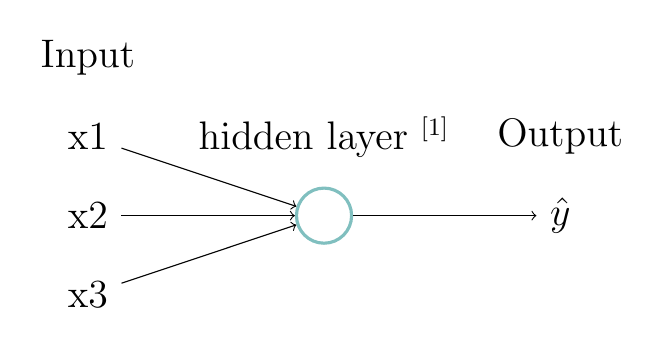
\begin{tikzpicture}
    % Input Layer
    \foreach \name/\i in {x1/1,x2/2,x3/3} {
        \node (Input-\i) at (0,-\i) {\name};
        \ifnum \i=1
            \node[above of=Input-\i] {Input};
        \fi
    }
    % Hidden Layer
    \foreach \i in {1} {
        \node[circle, minimum size = 7mm, draw=teal!50, line width=.4mm] (Hidden1-\i) at (3,-2) {};
        \ifnum \i=1
        \node[above of=Hidden1-\i] {hidden layer $^{[1]}$};
        \fi
    }
    % Output Layer
    \foreach \name/\i in {$\hat{y}$/1} {
        \node (Output-\i) at (6,-2) {\name};
        \ifnum \i=1
        \node[above of=Output-\i] {Output};
        \fi
    }
    % Arrows
    \foreach \i in {1,2,3} {
        \foreach \j in {1} {
           \draw[->] (Input-\i) -- (Hidden1-\j);
        }
    }
    \foreach \i in {1} {
        \foreach \j in {1} { \draw[->] (Hidden1-\i) -- (Output-\j);
        }
    }
\end{tikzpicture}


$\fbox{$x, w, b$} \rightarrow \fbox{$z=w^T x + b$} \rightarrow \fbox{$a=\sigma(z)$} $\\\\


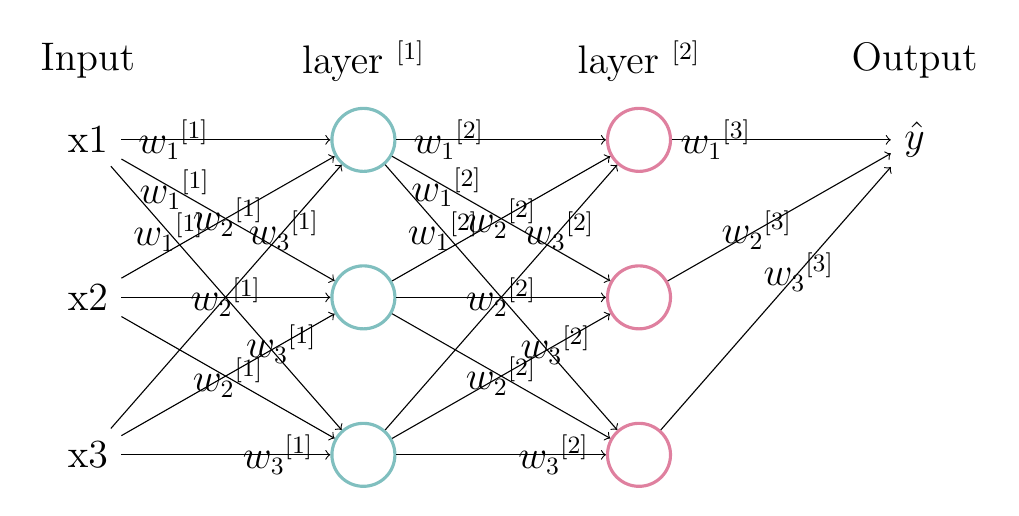
\begin{tikzpicture}
    % Input Layer
    \foreach \name/\i in {x1/1,x2/2,x3/3} {
        \node (Input-\i) at (0,-\i*2) {\name};
        \ifnum \i=1
            \node[above of=Input-\i] {Input};
        \fi
    }
    % Hidden Layer
    \foreach \i in {1,2,3} {
        \node[circle, minimum size = 8mm,draw=teal!50, line width=.4mm]
        (Hidden1-\i) at (3.5,-\i*2) {};
        \ifnum \i=1
        \node[above of=Hidden1-\i] {layer $^{[1]}$};
        \fi
    }
    \foreach \i in {1,2,3} {
        \node[circle, minimum size = 8mm, draw=purple!50, line width=.4mm]
        (Hidden2-\i) at (7,-\i*2) {};
        \ifnum \i=1
        \node[above of=Hidden2-\i] {layer $^{[2]}$};
        \fi
    }
    % Output Layer
    \foreach \name/\i in {$\hat{y}$/1} {
        \node (Output-\i) at (10.5,-\i*2) {\name};
        \ifnum \i=1
        \node[above of=Output-\i] {Output};
        \fi
    }
    % Arrows
    \foreach \i in {1,2,3} {
        \foreach \j in {1,2,3} {
           \draw[->] (Input-\i) -- (Hidden1-\j) node[pos=\i/4]{${w_\i}^{[1]}$};
        }
    }
    \foreach \i in {1,2,3} {
        \foreach \j in {1,2,3} {
           \draw[->] (Hidden1-\i) -- (Hidden2-\j) node[pos=\i/4]{${w_\i}^{[2]}$};
        }
    }
    \foreach \i in {1,2,3} {
        \foreach \j in {1} {
            \draw[->] (Hidden2-\i) -- (Output-\j) node[pos=\i/5]{${w_\i}^{[3]}$};
        }
    }
\end{tikzpicture}


$Layer^{[1]}: \fbox{$X, W^{[1]}, b^{[1]}$} \rightarrow \fbox{$Z^{[1]} = W^{[1]} X + b^{[1]}$} \rightarrow \fbox{$A^{[1]} = \sigma(Z^{[1]})$}$\\

$Layer^{[2]}: \fbox{$Z^{[2]} = W^{[2]} X + b^{[2]}$} \rightarrow \fbox{$A^{[2]} = \sigma(Z^{[2]})$} \rightarrow \fbox{$\mathcal{L}(A^{[2]},Y)$} $\\


\newpage
\subsection{Neural Network Representations}

Values of the input features (activation): $ X = a^{[0]}$\\

The following is the 2-Layer Neural Network:\\

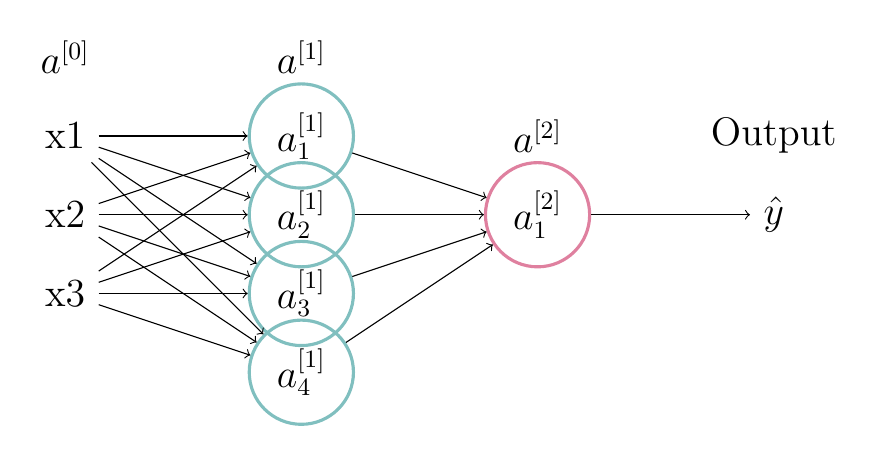
\begin{tikzpicture}
    % Input Layer
    \foreach \name/\i in {x1/1,x2/2,x3/3} {
        \node (Input-\i) at (0,-\i) {\name};
        \ifnum \i=1
            \node[above of=Input-\i] {$a^{[0]}$};
        \fi
    }
    % Hidden Layer
    \foreach \i in {1,2,3,4} {
        \node[circle, minimum size = 6mm, draw=teal!50, line width=.4mm] (Hidden1-\i) at (3,-\i) {$a_{\i}^{[1]}$};
        \ifnum \i=1
        \node[above of=Hidden1-\i] {$a^{[1]}$};
        \fi
    }
    \foreach \i in {1} {
        \node[circle, minimum size = 6mm, draw=purple!50, line width=.4mm] (Hidden2-\i) at (6,-2) {$a_{\i}^{[2]}$};
        \ifnum \i=1
        \node[above of=Hidden2-\i] {$a^{[2]}$};
        \fi
    }
    % Output Layer
    \foreach \name/\i in {$\hat{y}$/1} {
        \node (Output-\i) at (9,-2) {\name};
        \ifnum \i=1
        \node[above of=Output-\i] {Output};
        \fi
    }
    % Arrows
    \foreach \i in {1,2,3} {
        \foreach \j in {1,2,3,4} {
           \draw[->] (Input-\i) -- (Hidden1-\j);
        }
    }
    \foreach \i in {1,2,3,4} {
        \foreach \j in {1} {
           \draw[->] (Hidden1-\i) -- (Hidden2-\j);
        }
    }
    \foreach \i in {1} {
        \foreach \j in {1} {
            \draw[->] (Hidden2-\i) -- (Output-\j);
        }
    }
\end{tikzpicture}

${w^{[1]}}^T$ in $(4,3)$, $b^{[1]}$ in $(4,1)$\\

${w^{[2]}}^T$ in $(1,4)$, $b^{[2]}$ in $(1,1)$\\

\newpage
\subsection{Computing Neural Network Output}

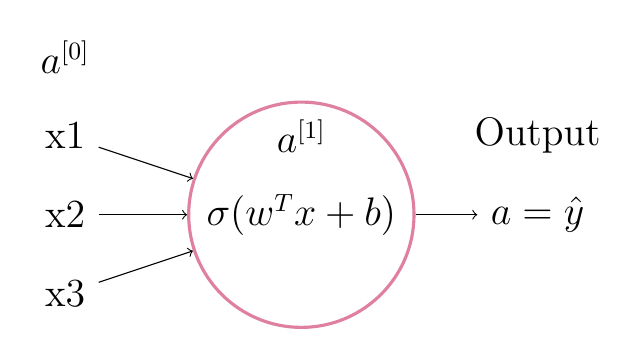
\begin{tikzpicture}
    % Input Layer
    \foreach \name/\i in {x1/1,x2/2,x3/3} {
        \node (Input-\i) at (0,-\i) {\name};
        \ifnum \i=1
            \node[above of=Input-\i] {$a^{[0]}$};
        \fi
    }
    % Hidden Layer
    \foreach \i in {1} {
        \node[circle, minimum size = 6mm, draw=purple!50, line width=.4mm] (Hidden1-\i) at (3,-2) {$\sigma(w^T x + b)$};
        \ifnum \i=1
        \node[above of=Hidden1-\i] {$a^{[1]}$};
        \fi
    }
    % Output Layer
    \foreach \name/\i in {$a=\hat{y}$/1} {
        \node (Output-\i) at (6,-2) {\name};
        \ifnum \i=1
        \node[above of=Output-\i] {Output};
        \fi
    }
    % Arrows
    \foreach \i in {1,2,3} {
        \foreach \j in {1} {
           \draw[->] (Input-\i) -- (Hidden1-\j);
        }
    }
    \foreach \i in {1} {
        \foreach \j in {1} {
            \draw[->] (Hidden1-\i) -- (Output-\j);
        }
    }
\end{tikzpicture}

Each circle(node) represents 2 steps of calculation:\\

$\fbox{$z = w^T x + b$}$\\

$\fbox{$a = \sigma(z)$}$\\

$\noindent\fbox{
\parbox{\textwidth}{
1. The weighted sum of the inputs is calculated.\\
2. The bias is added.\\
3. The result is fed to an activation function.\\
4. Specific neuron is activated.
    }
}$\\


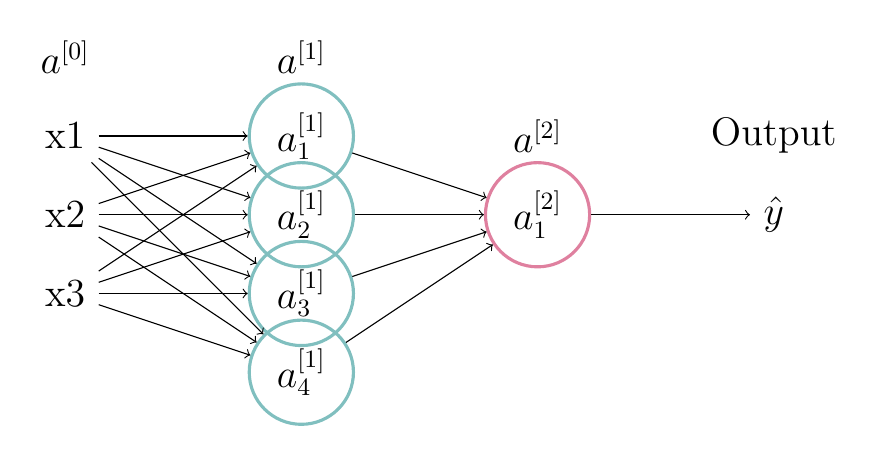
\begin{tikzpicture}
    % Input Layer
    \foreach \name/\i in {x1/1,x2/2,x3/3} {
        \node (Input-\i) at (0,-\i) {\name};
        \ifnum \i=1
            \node[above of=Input-\i] {$a^{[0]}$};
        \fi
    }
    % Hidden Layer
    \foreach \i in {1,2,3,4} {
        \node[circle, minimum size = 6mm, draw=teal!50, line width=.4mm] (Hidden1-\i) at (3,-\i) {$a_{\i}^{[1]}$};
        \ifnum \i=1
        \node[above of=Hidden1-\i] {$a^{[1]}$};
        \fi
    }
    \foreach \i in {1} {
        \node[circle, minimum size = 6mm, draw=purple!50, line width=.4mm] (Hidden2-\i) at (6,-2) {$a_{\i}^{[2]}$};
        \ifnum \i=1
        \node[above of=Hidden2-\i] {$a^{[2]}$};
        \fi
    }
    % Output Layer
    \foreach \name/\i in {$\hat{y}$/1} {
        \node (Output-\i) at (9,-2) {\name};
        \ifnum \i=1
        \node[above of=Output-\i] {Output};
        \fi
    }
    % Arrows
    \foreach \i in {1,2,3} {
        \foreach \j in {1,2,3,4} {
           \draw[->] (Input-\i) -- (Hidden1-\j);
        }
    }
    \foreach \i in {1,2,3,4} {
        \foreach \j in {1} {
           \draw[->] (Hidden1-\i) -- (Hidden2-\j);
        }
    }
    \foreach \i in {1} {
        \foreach \j in {1} {
            \draw[->] (Hidden2-\i) -- (Output-\j);
        }
    }
\end{tikzpicture}

$z_{1}^{[1]} = {w_{1}^{[1]}}^T X + b_{1}^{[1]}\hspace{3mm} \rightarrow\hspace{2mm} a_{1}^{[1]} = \sigma(z_{1}^{[1]})$\\

$z_{2}^{[1]} = {w_{2}^{[1]}}^T X + b_{2}^{[1]}\hspace{3mm} \rightarrow\hspace{2mm} a_{2}^{[1]} = \sigma(z_{2}^{[1]})$, \hspace{2mm} where $a_{i \hspace{4mm}\leftarrow \text{node in layer}}^{[l] \hspace{3mm}\leftarrow \text{layer}}$\\

$z^{[1]}=
\begin{bmatrix}
{w_{1}^{[1]}}^T X +b_{1}^{[1]} \\
{w_{2}^{[1]}}^T X +b_{2}^{[1]} \\
{w_{3}^{[1]}}^T X +b_{3}^{[1]} \\
{w_{4}^{[1]}}^T X +b_{4}^{[1]} \\
\end{bmatrix}
\hspace{3mm} \rightarrow
\hspace{3mm}
\begin{bmatrix}
\sigma({w_{1}^{[1]}}^T X +b_{1}^{[1]}) \\
\sigma({w_{2}^{[1]}}^T X +b_{2}^{[1]}) \\
\sigma({w_{3}^{[1]}}^T X +b_{3}^{[1]}) \\
\sigma({w_{4}^{[1]}}^T X +b_{4}^{[1]}) \\
\end{bmatrix}$\\


$a^{[1]} = \sigma(z^{[1]})=
\begin{bmatrix}
\sigma(z_{1}^{[1]}) \\
\sigma(z_{2}^{[1]}) \\
\sigma(z_{3}^{[1]}) \\
\sigma(z_{4}^{[1]}) \\
\end{bmatrix} =
\sigma[
\begin{bmatrix}
\dots & {w_{1}^{[1]}}^T & \dots \\
\dots & {w_{2}^{[1]}}^T & \dots \\
\dots & {w_{3}^{[1]}}^T & \dots \\
\dots & {w_{4}^{[1]}}^T & \dots \\
\end{bmatrix}
\begin{bmatrix}
x_{1} \\
x_{2} \\
x_{3} \\
\end{bmatrix} +
\begin{bmatrix}
b_{1}^{[1]} \\
b_{2}^{[1]} \\
b_{3}^{[1]} \\
b_{4}^{[1]} \\
\end{bmatrix}
]
$\\

\newpage


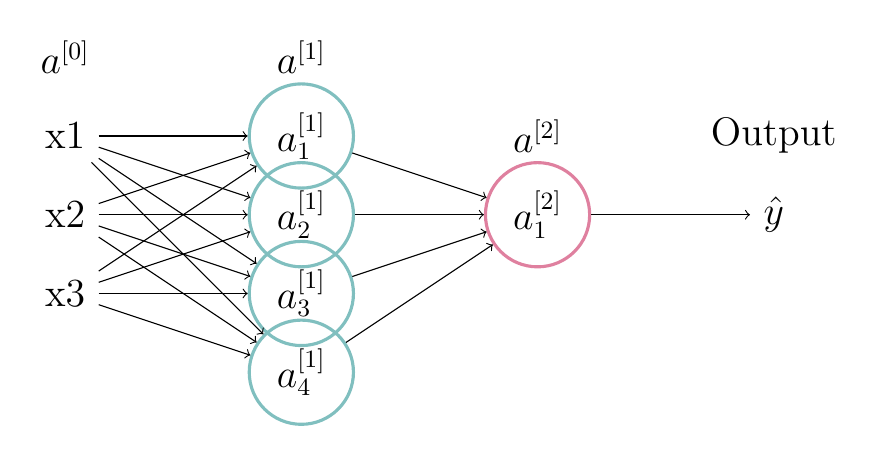
\begin{tikzpicture}
    % Input Layer
    \foreach \name/\i in {x1/1,x2/2,x3/3} {
        \node (Input-\i) at (0,-\i) {\name};
        \ifnum \i=1
            \node[above of=Input-\i] {$a^{[0]}$};
        \fi
    }
    % Hidden Layer
    \foreach \i in {1,2,3,4} {
        \node[circle, minimum size = 6mm, draw=teal!50, line width=.4mm] (Hidden1-\i) at (3,-\i) {$a_{\i}^{[1]}$};
        \ifnum \i=1
        \node[above of=Hidden1-\i] {$a^{[1]}$};
        \fi
    }
    \foreach \i in {1} {
        \node[circle, minimum size = 6mm, draw=purple!50, line width=.4mm] (Hidden2-\i) at (6,-2) {$a_{\i}^{[2]}$};
        \ifnum \i=1
        \node[above of=Hidden2-\i] {$a^{[2]}$};
        \fi
    }
    % Output Layer
    \foreach \name/\i in {$\hat{y}$/1} {
        \node (Output-\i) at (9,-2) {\name};
        \ifnum \i=1
        \node[above of=Output-\i] {Output};
        \fi
    }
    % Arrows
    \foreach \i in {1,2,3} {
        \foreach \j in {1,2,3,4} {
           \draw[->] (Input-\i) -- (Hidden1-\j);
        }
    }
    \foreach \i in {1,2,3,4} {
        \foreach \j in {1} {
           \draw[->] (Hidden1-\i) -- (Hidden2-\j);
        }
    }
    \foreach \i in {1} {
        \foreach \j in {1} {
            \draw[->] (Hidden2-\i) -- (Output-\j);
        }
    }
\end{tikzpicture}

Given input $x$:\\

$z^{[1]} = W^{[1]} a^{[0]} + b^{[1]}$, where $_{(4,1) = (4,3)(3,1)+ (4,1)}$\\

$a^{[1]} = \sigma(z^{[1]})$\\

$z^{[2]} = W^{[2]}a^{[1]} + b^{[2]}$, where $_{(1,1) = (1,4)(4,1)+ (1,1)}$\\

$a^{[2]} = \sigma(z^{[2]})$\\

\newpage
\subsection{Vectorizing Across Multiple Examples}

$x^{(i)} \hspace{2mm}\rightarrow \hspace{2mm} a^{[2](i)}= \hat{y}^{(i)}$\\

for $i=1$  to $m$:\\

$z^{[1](i)} = W^{[1]} x^{(i)} + b^{[1]}$\\

$a^{[1](i)} = \sigma(z^{[1](i)})$\\

$z^{[2](i)} = W^{[2]}a^{[1](i)} + b^{[2]}$\\

$a^{[2](i)} = \sigma(z^{[2](i)})$\\\\

For $m$ examples:\\

$X=
\begin{bmatrix}
    | & | & | & | \\
    X^{(1)} & X^{(2)} & \dots & X^{(m)} \\
    | & | & | & | \\
\end{bmatrix}$\\

$Z^{[1]}=
\begin{bmatrix}
    | & | & | & | \\
    z^{[1](1)} & z^{[1](2)} & \dots & z^{[1](m)} \\
    | & | & | & | \\
\end{bmatrix} = {W^{[1]}}^T X + b^{[1]}$\\

$A^{[1]}=
\begin{bmatrix}
    | & | & | & | \\
    a^{[1](1)} & a^{[1](2)} & \dots & a^{[1](m)} \\
    | & | & | & | \\
\end{bmatrix}
= \sigma(Z^{[1]}) = \sigma({W^{[1]}}^T X + b^{[1]})$\\


$\indent \updownarrow$: across hidden units in the $i^{th}$ training example; $\sharp$ of units/node \\

$\indent \leftrightarrow$: across $m$ training examples\\


\newpage
\subsection{Justification for vectorized implementation}

Given $m= 3$, let\\

$W^{[1]}X^{(1)}  =\begin{bmatrix}
    | \\
    $A$ \\
    | \\
\end{bmatrix}$, 
$W^{[1]}X^{(2)}  =\begin{bmatrix}
    | \\
    $B$ \\
    | \\
\end{bmatrix}$, 
$W^{[1]}X^{(3)}  =\begin{bmatrix}
    | \\
    $C$ \\
    | \\
\end{bmatrix}$\\

then, $Z^{[1]} = W^{[1]}\begin{bmatrix}
    | &| & | \\
    X^{(1)} & X^{(2)} & X^{(3)} \\
    | &| & | \\
\end{bmatrix}
=\begin{bmatrix}
    | & | & | \\
    A & B & C \\
    | & | & | \\
\end{bmatrix}
=\begin{bmatrix}
    | &| & | \\
    Z^{[1](1)} & Z^{[1](2)} & Z^{[1](3)} \\
    | &| & | \\
\end{bmatrix}
$\\

1. Using for-loops:\\

for $i=1$  to $m$:\\

$z^{[1](i)} = W^{[1]} x^{(i)} + b^{[1]}$\\

$a^{[1](i)} = \sigma(z^{[1](i)})$\\

$z^{[2](i)} = W^{[2]}a^{[1](i)} + b^{[2]}$\\

$a^{[2](i)} = \sigma(z^{[2](i)})$\\\\

2. Using Matrix(without for-loop): \\

Given X:\\

$Z^{[1]} = W^{[1]} X + b^{[1]}$\\

$A^{[1]} = \sigma(Z^{[1]})$\\

$Z^{[2]} = W^{[2]}A^{[1]} + b^{[2]}$\\

$A^{[2]} = \sigma(Z^{[2]})$\\\\



\newpage
\subsection{Activation Functions}

There're other activation functions other than sigmoid and you can use different activation functions for different layers; \\
$\sigma(z) \hspace{2mm} \rightarrow\hspace{2mm} g(z) = tanh(z) = \frac{e^{z} - e^{-z}}{e^{z}+e^{-z}}$\\

$tanh$ always works better on hidden layers than sigmoid function, except for output layer (use sigmoid for output layer) where it requires to output be either 0 or 1 (binary classification)\\


Use different activation functions $g^{[l]}(z^{[i]})$, where $l=1,2, \dots, L$ (number of layers in the network)


Both activation functions have down side; If z is either very small or large, the gradient(slope of the function) is very small which will slow down the gradient descent(backward propagation/learning speed).\\

ReLU function is a popular choice for the activation function; $a=max(0,z)$ that does not have above downsides.\\

In case of Binary Classification, use sigmoid for the output layer, and ReLu for other hidden layer's activation function. Or Leaky ReLU ($a=max(.01z, z)$) recently.(not commonly used in practice)\\

\newpage
\subsection{Why Non-linear Activation Functions}

Linear Activation through Hidden layers become meaningless.
Use $g(z)$ as non-linear function.\\
Using linear activation for hidden layers and sigmoid for the output layer will simply become a Logistic Regression problem..\\

\newpage
\subsection{Derivatives of Activation Functions.}

sigmoid activation function $g(z)= \frac{1}{1+e^{-z}}$ = a\\

$g^{'}(z)=\frac{d}{dz}g(z) =  g(z)(1-g(z)) = a(1-a)$\\

$tanh$ activation function $g(z)= tanh(z) = \frac{e^z-e^{-z}}{e^z+e^{-z}} = a$\\

$g^{'}(z)=1-(tanh(z))^2 = 1-a^2$\\

$ReLU$ activation function $g(z) = max(0,z)$\\

$g^{'}(z) = 0$ if $z < 0$\\

$g^{'}(z) = 1$ if $z \ge 0$\\

$Leaky ReLU$ activation function $g(z) = max(.01z,z)$\\

$g^{'}(z) = .01$ if $z<0$\\

$g^{'}(z) = 1$ if $z \ge 0$\\

\newpage
\subsection{Gradient Descent For Neural Networks}

Backward propagation.\\

Parameters:\\

$w^{[1]}$, $b^{[1]}$, $w^{[2]}$, $b^{[2]}$ matrices with dimensions:\\

$_{(n^{[1]}, n^{[0]})}$, $_{(n^{[1]}, 1)}$, $_{(n^{[2]}, n^{[1]})}$, $_{(n^{[2]}, 1)}$, where \\

$_{n_x = n^{[0]}=\text{num of input features}}$, $_{n^{[1]}= \text{num of hidden units}}$, $_{n^{[2]}=1=\text{num of output units}}$\\

Cost Funcion:\\

$\hspace{4mm} J(w^{[1]}, b^{[1]}, w^{[2]}, b^{[2]}) = \frac{1}{m} \sum_{i=1}^m \mathcal{L}(\hat{y}, y)$, where $\hat{y}=a^{[2]}$\\


Gradien Descent:\\

$\noindent\fbox{
\parbox{\textwidth}{

Repeat:\\
$\indent$ Compute predicts ${\hat{y}}^{(i)}$ for $i=1,...,m$\\
$\indent$ $\indent$ $dw^{[1]} = \frac{\partial J}{\partial w^{[1]}}$, $db^{[1]} = \frac{\partial J}{\partial b^{[1]}}$\\
$\indent$ $\indent$ $w^{[1]} := w^{[1]} -\alpha dw^{[1]}$\\
$\indent$ $\indent$ $b^{[1]} := b^{[1]} -\alpha db^{[1]}$\\
$\indent$ $\indent$ $w^{[2]} := w^{[2]} -\alpha dw^{[2]}$\\
$\indent$ $\indent$ $b^{[2]} := b^{[2]} -\alpha db^{[2]}$\\

}
}$\\

\newpage

\textbf{Formulas for computing derivatives:}\\

Forward propagtion:\\

$Z^{[1]} = W^{[1]} X + b^{[1]}$\\

$A^{[1]} = g^{[1]}(Z^{[1]})$\\

$Z^{[2]} = W^{[2]} A^{[1]} + b^{[2]}$\\

$A^{[2]} = g^{[2]}(Z^{[2]}) = \sigma(Z^{[2]})$, sigmoid for binary classification.\\


Backward propagtion:\\

$dZ^{[2]} = A^{[2]} - Y = [y^{(1)}, \dots,y^{(m)}]$\\

$dW^{[2]} = \frac{1}{m}dZ^{[2]} {A^{[1]}}^T$\\

$db^{[2]} = \frac{1}{m}$ np.sum$(dZ^{[2]}, axis=1, keepdims=True)$\\

    , where keepdims ensures $(n^{[2]}, 1)$ instead of $(n,)$\\

$dZ^{[1]} ={W^{[2]}}^T dZ^{[2]} * {g^{[1]}}^{'} (Z^{[1]})$; elementwise product in $_{(n^{[1]}, m)}$\\

$dW^{[1]} = \frac{1}{m}dZ^{[1]}X^T$\\

$db^{[1]} = \frac{1}{m}$ np.sum$(dZ^{[1]}, axis=1, keepdims=True)$\\


\newpage
\subsection{BackPropagation Intuition}

Logistic Regression Recap\\

Forward Propagation in Logistic Regression:\\

\begin{tikzpicture}
    % Input Layer
    \foreach \name/\i in {$x$/1,$w$/2,$b$/3} {
        \node (Input-\i) at (0,-\i) {\name};
        \ifnum \i=1
            \node[above of=Input-\i] {};
        \fi
    }
    % Hidden Layer
    \foreach \i in {1} {
        \node (Hidden1-\i) at (3,-2) {$\fbox{$z=w^T x + b$}$};
    }
    \foreach \i in {1} {
        \node (Hidden2-\i) at (6,-2) {$\fbox{$a=\sigma(z)$}$};
    }
    % Output Layer
    \foreach \i in {1} {
        \node (Output-\i) at (9,-2) {$\mathcal{L}(a,y)$};
    }
    % Arrows
    \foreach \i in {1,2,3} {
        \foreach \j in {1} {
           \draw[->] (Input-\i) -- (Hidden1-\j);
        }
    }
    \foreach \i in {1} {
        \foreach \j in {1} {
           \draw[->] (Hidden1-\i) -- (Hidden2-\j);
        }
    }
    \foreach \i in {1} {
        \foreach \j in {1} { \draw[->] (Hidden2-\i) -- (Output-\j);
        }
    }
\end{tikzpicture}

Backward Propagation in Logistic Regression:\\

$da = \frac{d}{da}\mathcal{L}(a,y) = \frac{d}{da}[-y\log{a} -(1-y)\log(1-a)]=-\frac{y}{a} +\frac{1-y}{1-a} = \frac{a-y}{a(1-a)}$\\

$dz = \frac{d}{dz}\mathcal{L}(a,y) = \frac{d}{da}\mathcal{L}(a,y) \frac{dz}{da}= da \cdot \frac{dz}{da} = da \cdot g^{'}(z)$\\

,$\hspace{2mm} _{\text{where} \hspace{1mm} a=g(z) \hspace{1mm}\text{and therefore\hspace{1mm}} \frac{dz}{da} = g^{'}(z) \hspace{1mm} \text{In case of logistic regression: } g(z) = \sigma(z), \text{therefore } g^{'}(z) = g(z)(1-g(z))}$\\

$dw = \frac{d}{dz}\mathcal{L}(a,y) \frac{dz}{dw} = dz\cdot x$\\

$db = \frac{d}{dz}\mathcal{L}(a,y) \frac{dz}{db} = dz$\\


\newpage

Neural network gradients:\\

Compute forward:\\

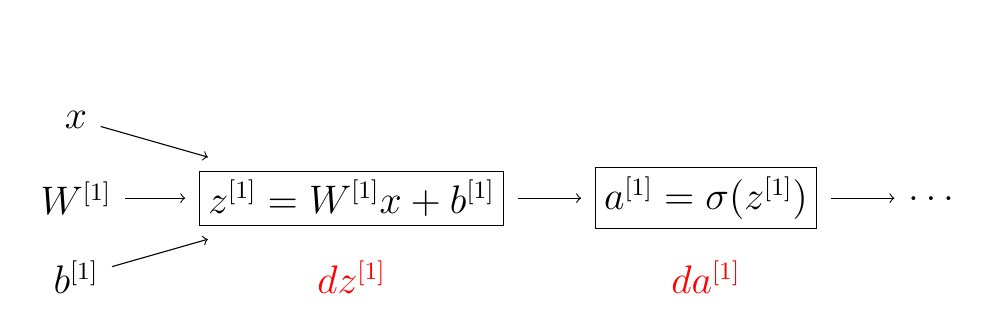
\begin{tikzpicture}
    % Input Layer
    \foreach \name/\i in {$x$/1,$W^{[1]}$/2,$b^{[1]}$/3} {
        \node (Input-\i) at (0,-\i) {\name};
        \ifnum \i=1
            \node[above of=Input-\i] {};
        \fi
    }
    % Hidden Layer
    \foreach \i in {1} {
        \node (Hidden1-\i) at (3.5,-2) {$\fbox{$z^{[1]}=W^{[1]} x + b^{[1]}$}$};
        \node[below of=Hidden1-\i] {$\textcolor{red}{dz^{[1]}}$};
    }
    \foreach \i in {1} {
        \node (Hidden2-\i) at (8,-2) {$\fbox{$a^{[1]}=\sigma(z^{[1]})$}$};
        \node[below of=Hidden2-\i] {$\textcolor{red}{da^{[1]}}$};
    }
    \foreach \i in {1} {
        \node (Hidden3-\i) at (10.9,-2) {$\dots$};
    }
    % Arrows
    \foreach \i in {1,2,3} {
        \foreach \j in {1} {
           \draw[->] (Input-\i) -- (Hidden1-\j);
        }
    }
    \foreach \i in {1} {
        \foreach \j in {1} {
           \draw[->] (Hidden1-\i) -- (Hidden2-\j);
        }
    }
    \foreach \i in {1} {
        \foreach \j in {1} {
           \draw[->] (Hidden2-\i) -- (Hidden3-\j);
        }
    }
\end{tikzpicture}


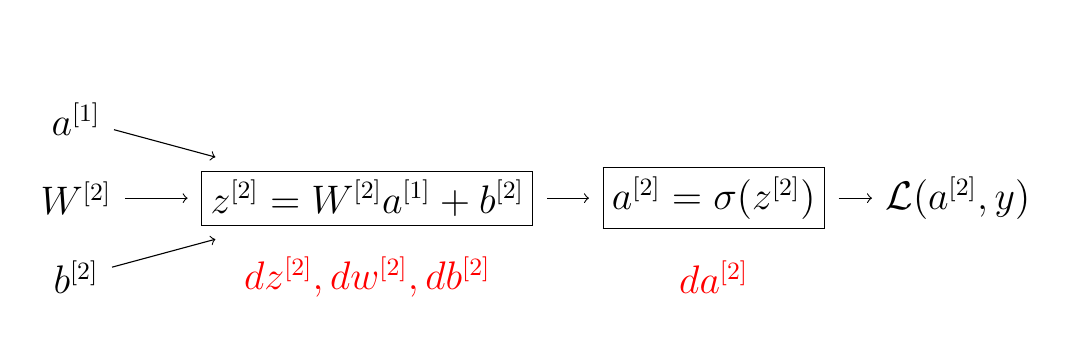
\begin{tikzpicture}
    % Hidden Layer
    \foreach \i in {1} {
        \node (Hidden2-\i) at (0,-2) {};
    }
    \foreach \name/\i in {$a^{[1]}$/1,$W^{[2]}$/2,$b^{[2]}$/3} {
        \node (Hidden2-\i) at (0,-\i) {\name};
        \ifnum \i=1
            \node[above of=Hidden2-\i] {};
        \fi
    }
    \foreach \i in {1} {
        \node (Hidden3-\i) at (3.7,-2) {$\fbox{$z^{[2]}=W^{[2]} a^{[1]} + b^{[2]}$}$};
        \node[below of=Hidden3-\i] {$\textcolor{red}{dz^{[2]}, dw^{[2]}, db^{[2]}}$};
    }
    \foreach \i in {1} {
        \node (Hidden4-\i) at (8.1,-2) {$\fbox{$a^{[2]}=\sigma(z^{[2]})$}$};
        \node[below of=Hidden4-\i] {$\textcolor{red}{da^{[2]}}$};
    }
    % Output Layer
    \foreach \i in {1} {
        \node (Output-\i) at (11.2,-2) {$\mathcal{L}(a^{[2]},y)$};
    }
    % Arrows
    \foreach \i in {1,2,3} {
        \foreach \j in {1} {
           \draw[->] (Hidden2-\i) -- (Hidden3-\j);
        }
    }
    \foreach \i in {1} {
        \foreach \j in {1} {
           \draw[->] (Hidden3-\i) -- (Hidden4-\j);
        }
    }
    \foreach \i in {1} {
        \foreach \j in {1} { \draw[->] (Hidden4-\i) -- (Output-\j);
        }
    }
\end{tikzpicture}


Compute backward ($n_x = n^{[0]}, n^{[1]}, n^{[2]}= 1$)\\

$da^{[2]} \rightarrow dz^{[2]} \rightarrow dw^{[2]}, db^{[2]} \rightarrow
da^{[1]} \rightarrow dz^{[1]} \rightarrow dw^{[1]}, db^{[1]}$\\

$\fbox{$dz^{[2]}$} = a^{[2]}-y \hspace{5mm}  _{\text{(logistic regression: activation for output layer is sigmoid)} \hspace{2mm} a^{[2]} = \sigma(z^{[2]})}$ \\

$\fbox{$dw^{[2]}$} = dz^{[2]} {a^{[1]}}^T \hspace{5mm} _{\text{(similar to logistic regression problem)}} \hspace{2mm} _{dw=dz\cdot x}$\\

$\fbox{$db^{[2]}$} = dz^{[2]}$\\

\noindent\rule{8cm}{0.4pt}


$\fbox{$dz^{[1]}$} = {w^{[2]}}^T dz^{[2]} * {g^{[1]}}^{'}(z^{[1]})$ where $_{(n^{[1]},1)} = _{(n^{[1]},n^{[2]})}  \cdot _{(n^{[2]}, 1)} * _{(n^{[1]}, 1)}$\\

$\fbox{$dw^{[1]}$} = dz^{[1]} {X}^T = dz^{[1]} {a^{[0]}}^T$\\

$\fbox{$db^{[1]}$} = dz^{[1]}$\\


\newpage

Summary of gradient descent\\

For a simple training example: (from the previouse slide)\\

$dz^{[2]} = a^{[2]} - y$\\

$dW^{[2]} = dz^{[2]} - {a^{[1]}}^T$\\

$db^{[2]} = dz^{[2]}$\\

$dz^{[1]} = {W^{[2]}}^T dz^{[2]} * {{g^{[1]}}}^{'}(z^{[1]})$\\

$dW^{[1]} = dz^{[1]}x^T$\\

$db^{[1]} = dz^{[1]}$\\

\noindent\rule{8cm}{0.4pt}

For $m$ training examples: \\

$dZ^{[2]} = A^{[2]} - Y$\\

$dW^{[2]} = \frac{1}{m}dZ^{[2]}{A^{[1]}}^T$\\

$db^{[2]} = \frac{1}{m}np.sum(dZ^{[2]}, axis=1, keepdims=True)$\\

$dZ^{[1]} = {W^{[2]}}^T dZ^{[2]} * {{g^{[1]}}}^{'}(Z^{[1]})$, elementwise in $_{(n^{[1]},m)}$ dimension.\\

$dW^{[1]} = \frac{1}{m} dZ^{[1]} X^T$\\

$db^{[1]} = \frac{1}{m}np.sum(dZ^{[1]}, axis=1, keepdims=True)$\\


\newpage
\subsection{Random Initialization}

What happens if you initialize weights to zero?\\

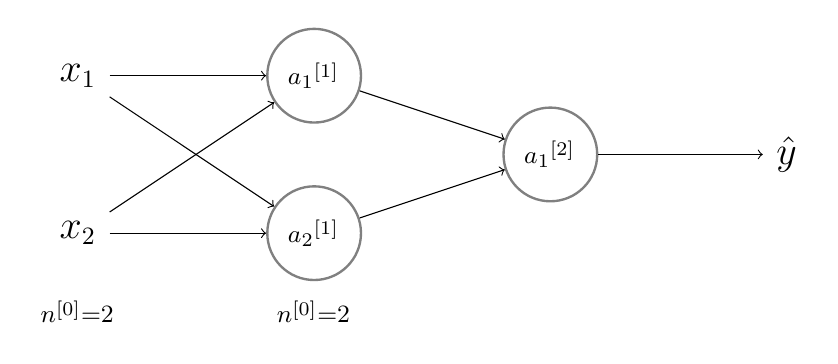
\begin{tikzpicture}
    % Input Layer
    \foreach \name/\i in {$x_1$/1,$x_2$/2} {
        \node (Input-\i) at (0,-\i*2) {\name};
        \ifnum \i=2
        \node[below of=Input-\i] {$_{n^{[0]}=2}$};
        \fi
    }
    % Hidden Layer
    \foreach \i in {1,2} {
        \node[circle, minimum size = 5mm, draw=black!50, line width=.3mm]
        (Hidden1-\i) at (3,-\i*2) {$_{{a_{\i}}^{[1]}}$};
        \ifnum \i=2
        \node[below of=Hidden1-\i] {$_{n^{[0]}=2}$};
        \fi
    }
    \foreach \i in {1} {
        \node[circle, minimum size = 5mm, draw=black!50, line width=.3mm]
        (Hidden2-\i) at (6,-3) {$_{{a_{\i}}^{[2]}}$};
        \ifnum \i=2
        \node[below of=Hidden2-\i] {$_{n^{[2]}=1}$};
        \fi
    }
    \foreach \i in {1} {
        \node (Output-\i) at (9,-3) {$\hat{y}$};
    }
    % Arrows
    \foreach \i in {1,2} {
        \foreach \j in {1,2} {
           \draw[->] (Input-\i) -- (Hidden1-\j);
        }
    }
    \foreach \i in {1,2} {
        \foreach \j in {1} {
           \draw[->] (Hidden1-\i) -- (Hidden2-\j);
        }
    }
    \foreach \i in {1} {
        \foreach \j in {1} {
           \draw[->] (Hidden2-\i) -- (Output-\j);
        }
    }
\end{tikzpicture}


$w^{[1]} = \begin{bmatrix}
   0 & 0 \\ 
   0 & 0 \\ 
\end{bmatrix}$, 
$b^{[1]} = \begin{bmatrix}
   0 \\ 
   0 \\ 
\end{bmatrix}$ gives $w^{[2]} = \begin{bmatrix}
   0 & 0\\ 
\end{bmatrix}$ and hidden units in $^{[1]}$ are identical. So having more than one hidden units become meaningless.\\

${a_1}^{[1]} = {a_2}^{[1]} $\\

${dz_1}^{[1]} = {dz_2}^{[1]} $\\


Random Initialization\\

$w^{[1]} = np.random.randn((2,2)) * \textcolor{blue}{.01}$\\

$b^{[1]} = np.zeros((2,1)) $\\

$w^{[2]} = np.random.randn((1,2)) * \textcolor{blue}{.01}$\\

$b^{[2]} = 0$\\

$_{\textcolor{blue}{\text{(big multiplier will make slope of the gradient descent is very small, so choose it as a small value.)}}}$\\


\end{document}

